%!TEX root = report.tex

For this exercise we created a new launch file \t{exercise5.launch}. In which we launch the scene with the closing doors from assignment 3b and all the other components that were used in this exercise, but with a separate set of parameters. The most important difference with the parameters in assignment 3b are the following lines:

\lstinputlisting[
	caption={Enabling topics},
	label={lst:5:topics}, 
	language=XML,
	firstline=43,
	lastline=44
]{./src/5/base_local_planner_params_ex5.yaml}

These parameters enable some topics that visualize the costmap and the trajectory analysis that the local planner does.
The experiments for this assignment can be launched with the following command:

\begin{lstlisting}
	roslaunch navigation exercise5.launch
\end{lstlisting}

After launching the experiments we also launched the tool \t{rqt_graph} which we used to visualize the velocities of the robot and the velocity that was sent to the robot through commands.

\begin{figure}
	\centering
	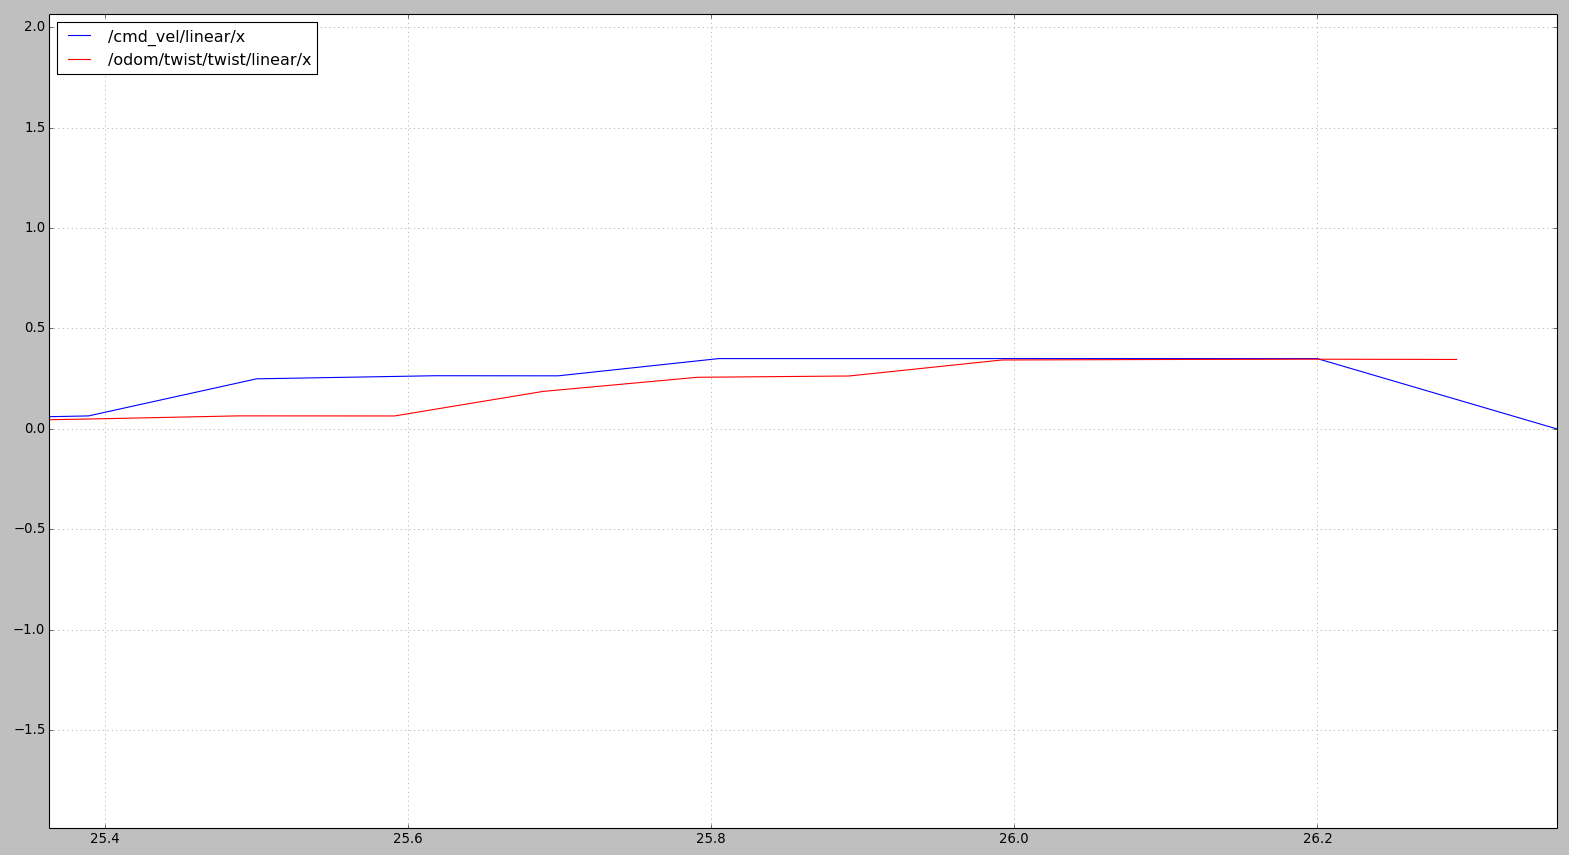
\includegraphics[width=0.80\textwidth]{./img/graph}
	\caption{Visualization of the linear command velocity \t{cmd_vel/linear/x} and the actual linear velocity \t{odom/twist/twist/linear/x} at a certain point in the simulation.}
	\label{fig:5:graph}
\end{figure}

From these graphs (\cref{fig:5:graph}) it became clear the it takes some time for the command to be executed by the robot as there is a slight delay between changes in the command velocity curve and the actual velocity curve.

We used this tool together with the new topics for visualization to analyse the effect of certain parameters for the local planner.

First we looked at the effects that the changes in the parameters for the angular and linear acceleration limits had on the behaviour of the robot. Slight changes in the angular limit parameter, \t{acc_lim_theta} had an effect on the range of angles that the local planner could simulate, see \cref{fig:5:acc_lim_theta}

\begin{figure}
	\centering
	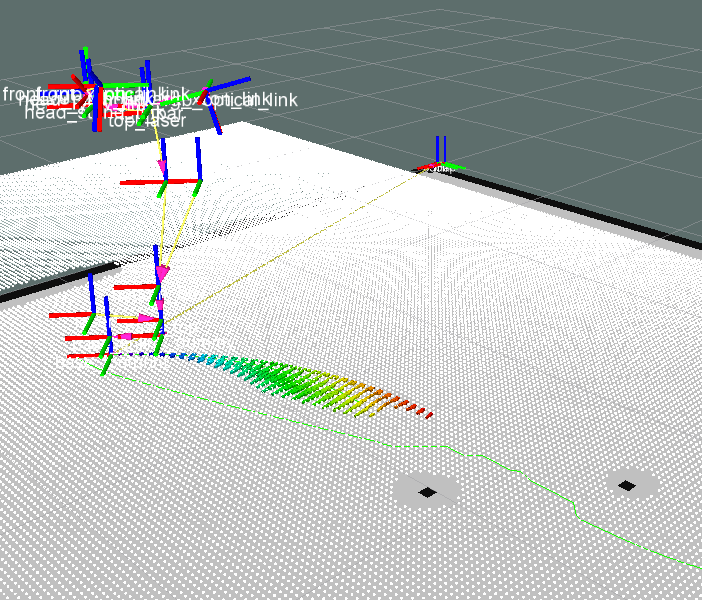
\includegraphics[width=0.46\textwidth]{./img/smallangularA}
	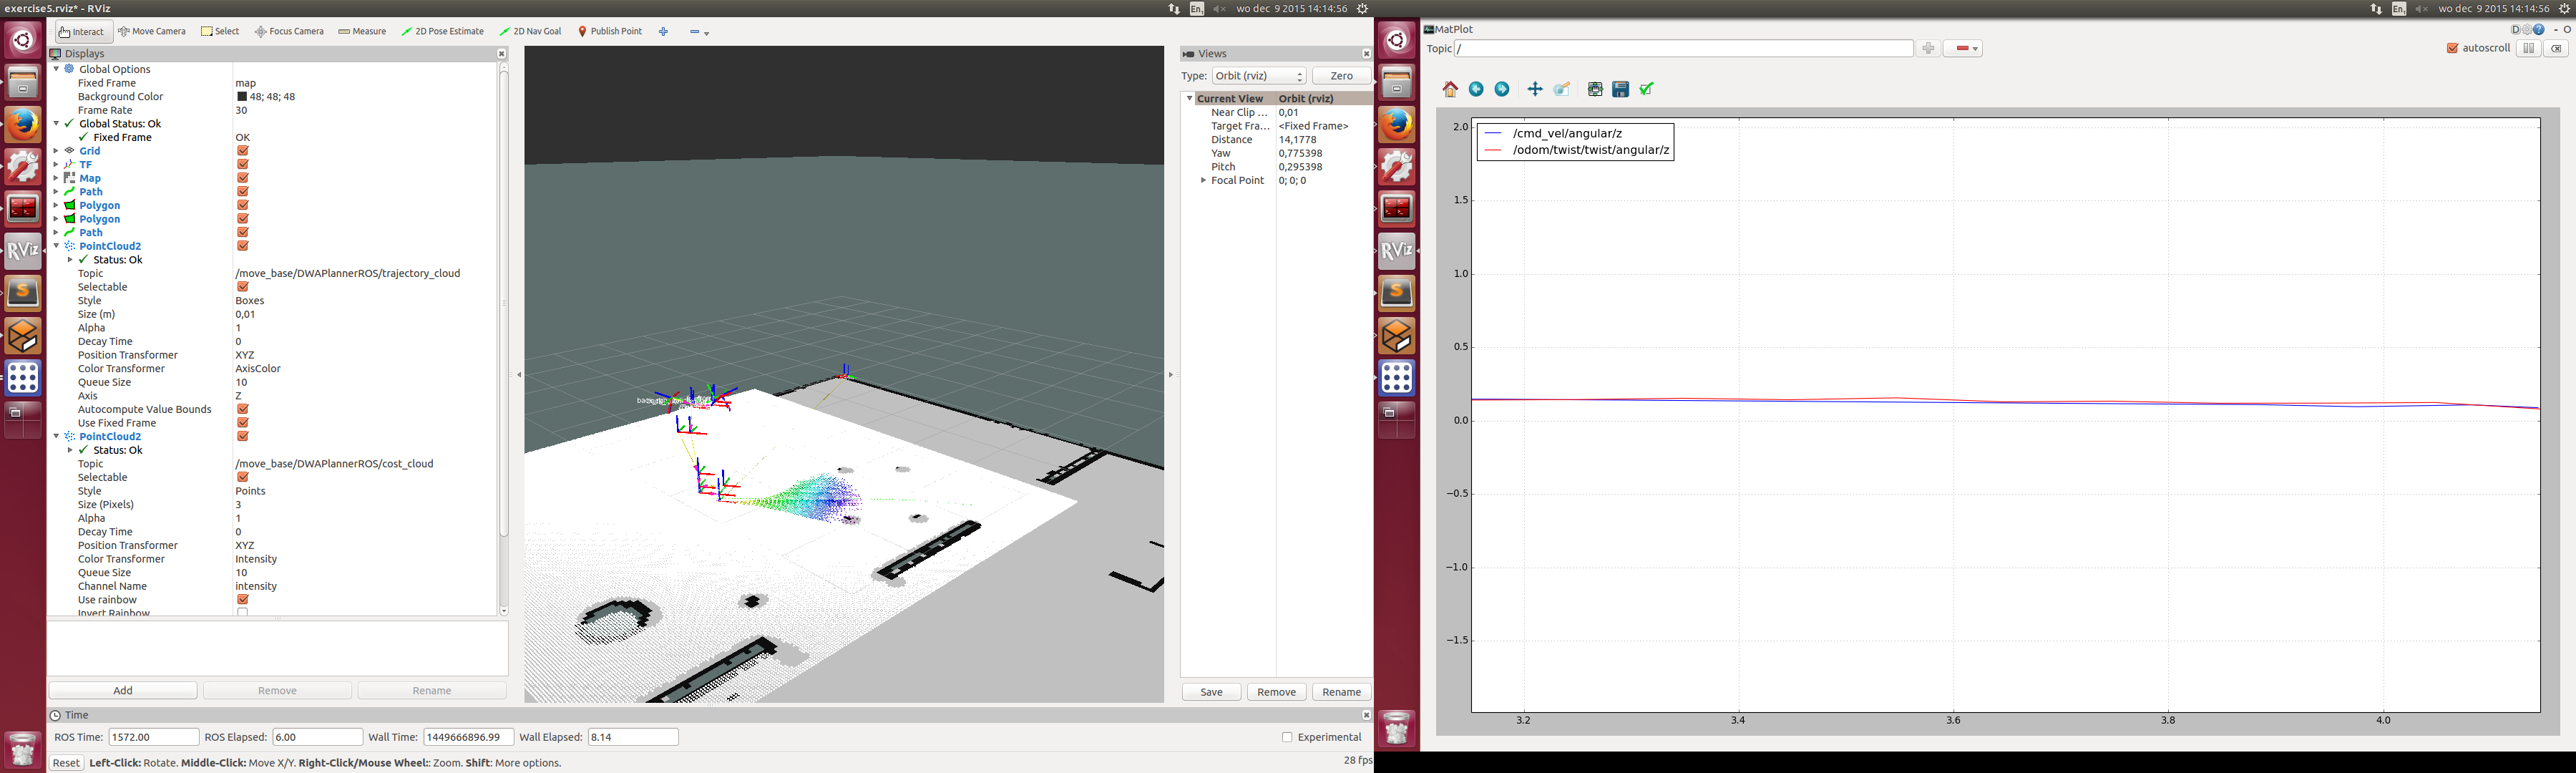
\includegraphics[width=0.46\textwidth]{./img/highangularA}
	\caption{The effect of varying the angular acceleration limit from low (left) to high (right) on the local planner.}
	\label{fig:5:acc_lim_theta}
\end{figure}

The images show that for a higher angular acceleration limit, the range of possible endpoints from local trajectories that are simulated by the planner is much wider than that of a lower limit. The effect of this in the simulation was that for lower limits the robot wasn't able to make sharp turns, but for a higher limit, the robot tended to make turns that were so sharp that the robot practically turned around an remained in almost the same position. We saw the robot make the most effective turns for an angular acceleration limit of 1.2.

As similar change of behaviour happened when changing \t{acc_lim_x}, the linear acceleration limit. See \cref{fig:5:acc_lim_x}.

\begin{figure}
	\centering
	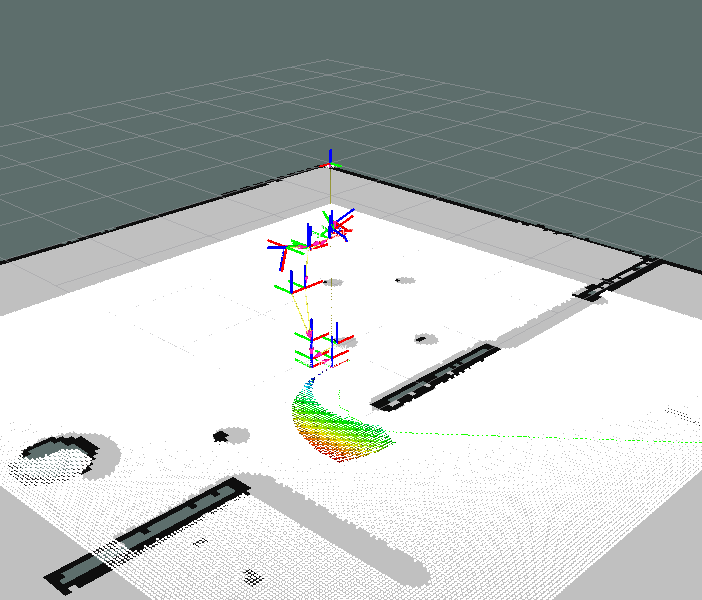
\includegraphics[width=0.46\textwidth]{./img/lowlinearA}
	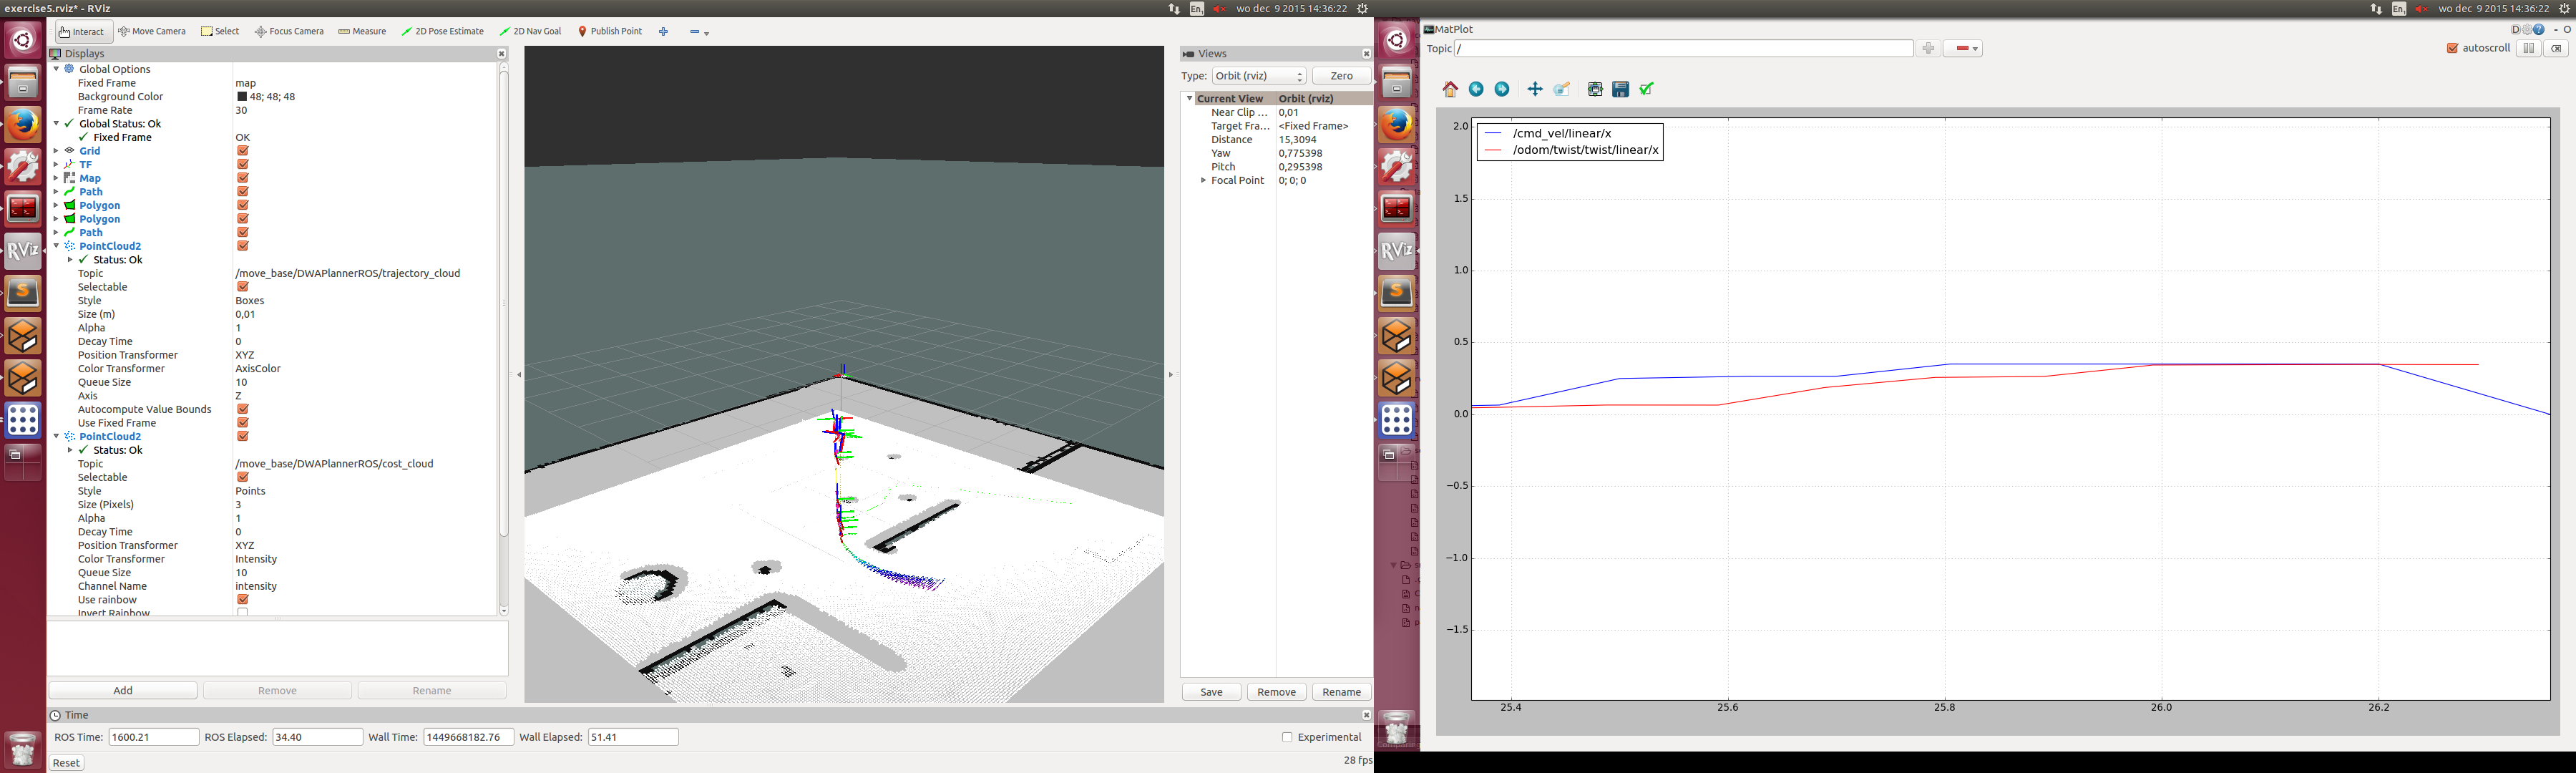
\includegraphics[width=0.46\textwidth]{./img/highlinearA}
	\caption{The effect of varying the linear acceleration limit from low (left) to high (right) on the local planner.}
	\label{fig:5:acc_lim_x}
\end{figure}

We were not able to vary the limit below 0.4, this prevented the robot from moving at all. When increasing the limit, the lengths of the simulated paths seemed to become longer at the costs of the width of the paths. With higher linear acceleration limit, the robot wasn't able to make sharp turns, this is why \t{acc_lim_x: 0.4} was optimal.

Furthermore, the sampling rates of the trajectory simulation can be changed with the \t{vth_samples} and \t{vx_samples} parameters. These parameters determine how many different angular velocities and linear velocities the local planner simulates. For higher values of these, the robot will find better trajectories, but will require more computations. Reducing these parameters will make the effect of this sampling visible, see \cref{fig:5:sampling}

\begin{figure}
	\centering
	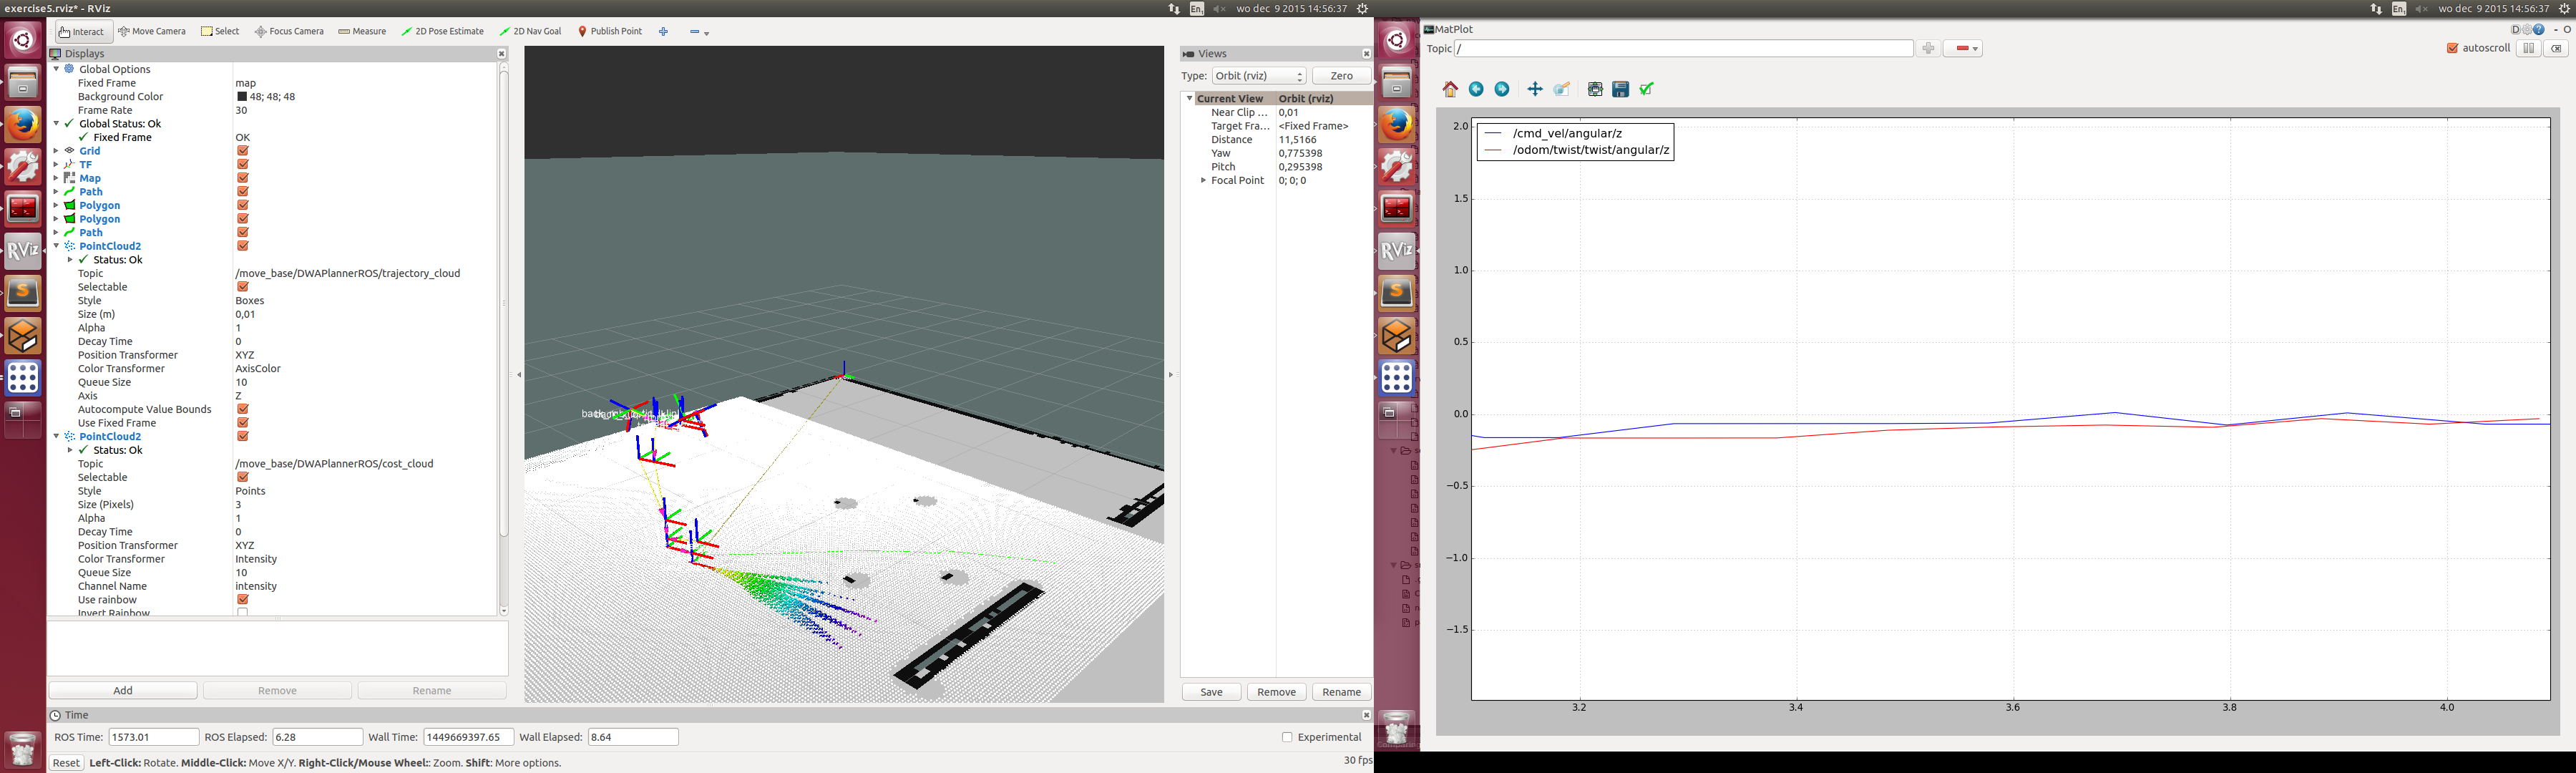
\includegraphics[width=0.46\textwidth]{./img/5samplingtheta}
	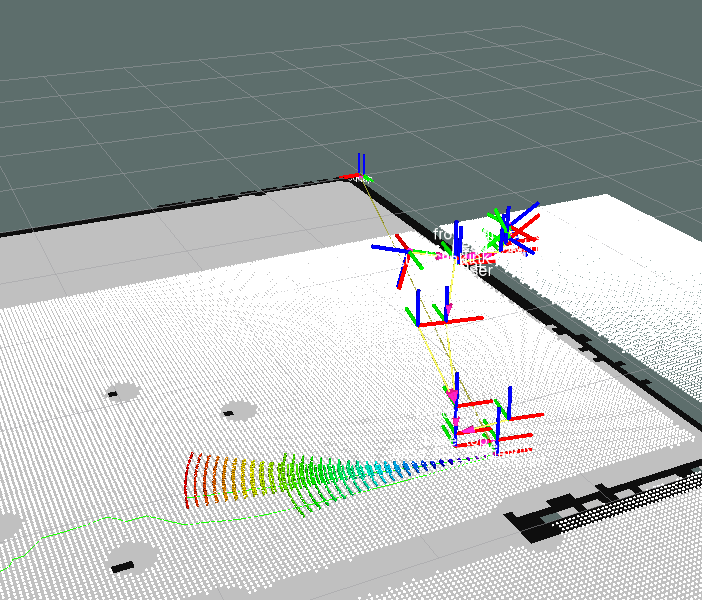
\includegraphics[width=0.46\textwidth]{./img/xsampling}
	\caption{Low sampling for the angular velocity (left) and the linear velocity (right).}
	\label{fig:5:sampling}
\end{figure}

Other important simulation parameters are \t{sim_time} and \t{sim_granularity}. That determine the time of each separate trajectory simulation and the distance between locations in the simulation respectively. The effect of this is shown in \cref{fig:5:sim}

\begin{figure}
	\centering
	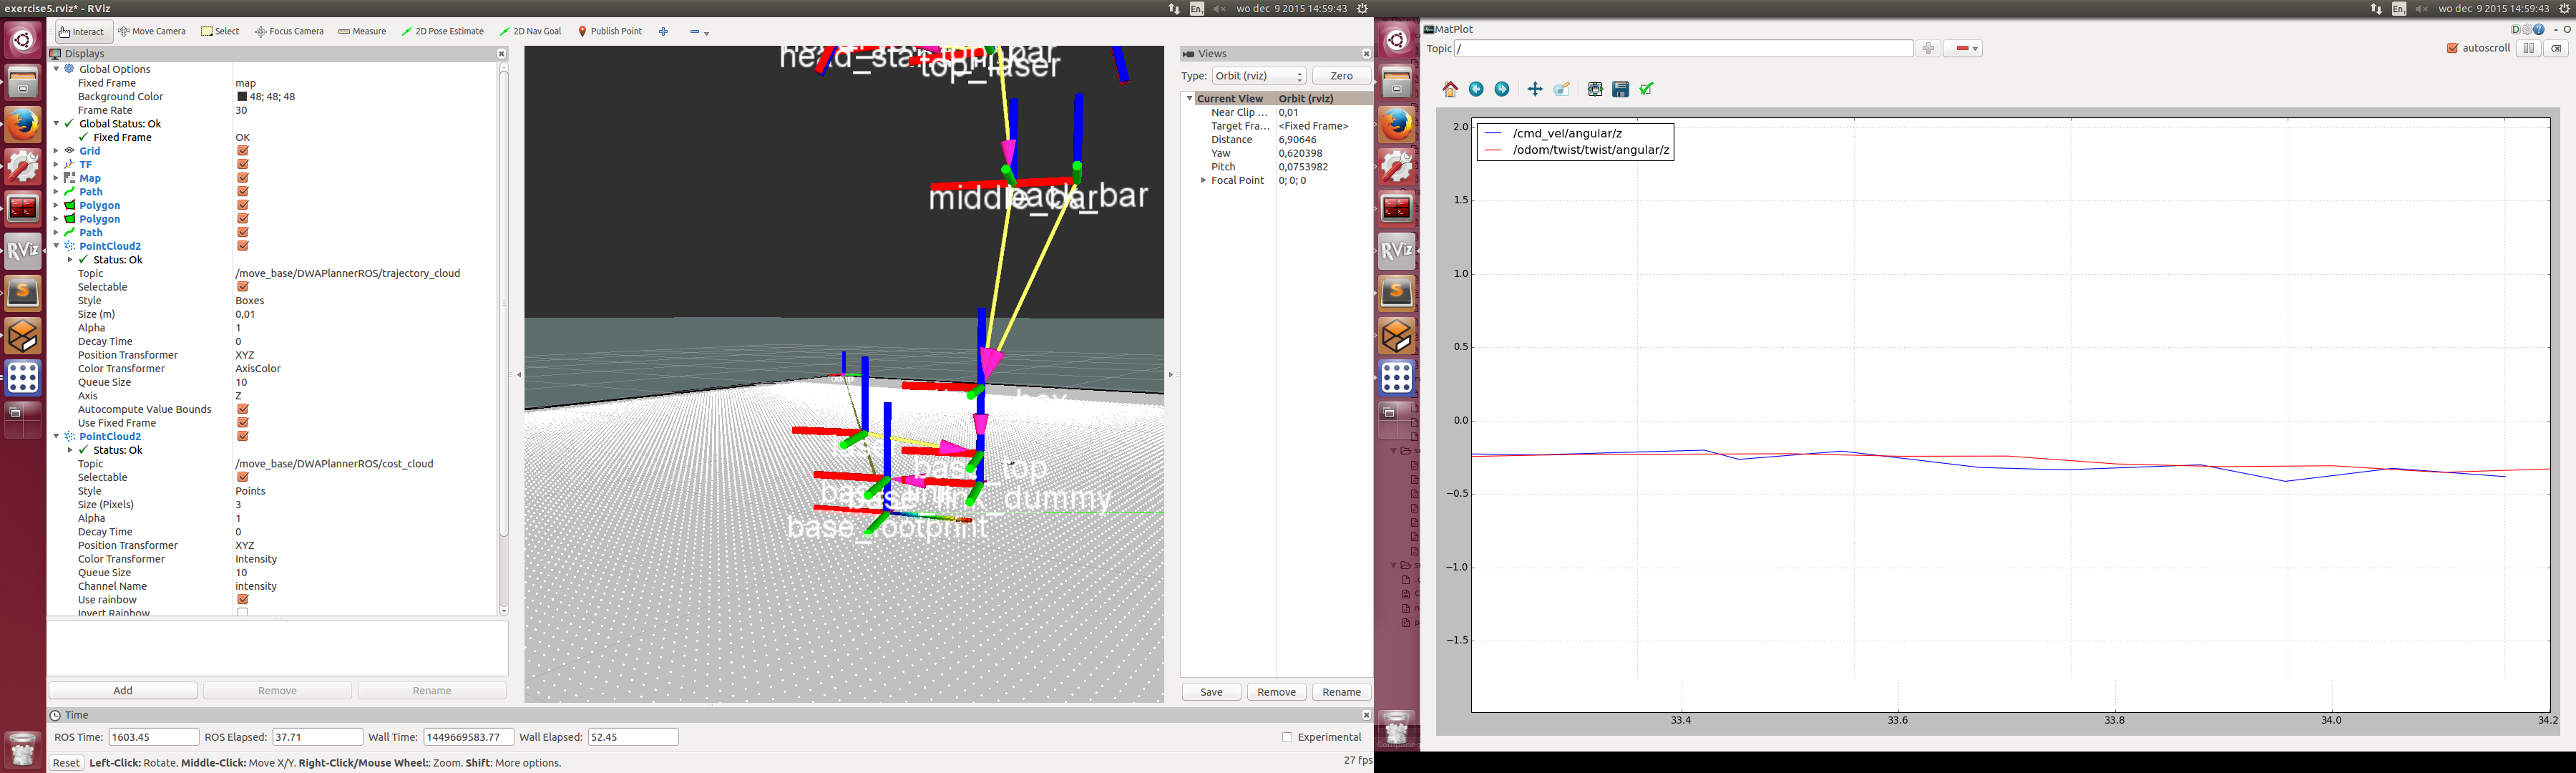
\includegraphics[width=0.46\textwidth]{./img/1simtime}
	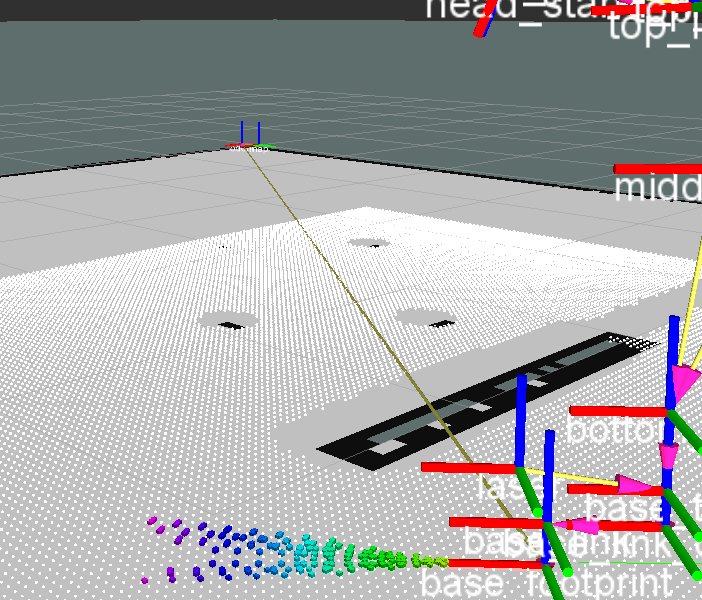
\includegraphics[width=0.46\textwidth]{./img/09granularity}
	\caption{Low simulation time (left) and low simulation granularity (right).}
	\label{fig:5:sim}
\end{figure}

Finally the are some parameters that have an influence on the score of each simulated trajectory. The main parameters for this are \t{goal_distance_bias}, \t{path_distance_bias} and \t{occdist_scale}. The score of a trajectory is calculated as follows \cite{ROSorg}:

\begin{quote}
\begin{lstlisting}[language = XML]
	cost =
  path_distance_bias * (distance to path from the endpoint of the trajectory in meters)
  + goal_distance_bias * (distance to local goal from the endpoint of the trajectory in meters)
  + occdist_scale * (maximum obstacle cost along the trajectory in obstacle cost (0-254))roslaunch navigation exercise5.launch
\end{lstlisting}
\end{quote}

